\documentclass[11pt,twocolumn]{article}
\usepackage{times}
\usepackage{graphicx}
\usepackage{amsmath}
\usepackage{hyperref}
\usepackage{listings}
\usepackage{xcolor}
\usepackage{float}
\usepackage{tikz}
\usepackage{booktabs}
\usepackage{geometry}
\usepackage{multicol}
\geometry{margin=0.75in}

\usetikzlibrary{shapes.geometric, arrows, positioning}

\title{\textbf{Enhancing LLM Inference with GraphRAG: \\A DSPy-Based Text2Cypher System}}
\author{Duong Ha, Khanh Tran}
\date{\today}

\begin{document}

\twocolumn[
\begin{@twocolumnfalse}
\maketitle
\begin{abstract}
Large Language Models (LLMs) excel at natural language understanding but lack reliable access to structured knowledge in graph databases. GraphRAG addresses this by translating natural language queries into Cypher, retrieving evidence from knowledge graphs, and generating grounded answers. However, standard Text2Cypher pipelines suffer from incorrect query generation, inefficient repeated computation, and lack of observability.

This work presents an enhanced GraphRAG system built on DSPy that implements: (1) dynamic few-shot exemplar selection using semantic similarity, (2) automated schema pruning for context optimization, (3) Cypher query validation with self-refinement loops, (4) LRU caching for query results, and (5) comprehensive performance benchmarking. Evaluated on a Nobel Prize knowledge graph with 726 scholars and 9 prize categories, the system achieves correct query generation and demonstrates up to 100\% cache hit rates for repeated queries. Performance profiling reveals schema pruning as the primary bottleneck (52-56\% of execution time), providing clear directions for future optimization.
\end{abstract}
\vspace{0.3cm}
\end{@twocolumnfalse}
]

\section{Introduction}
While LLMs demonstrate strong reasoning capabilities over unstructured text, they lack deterministic access to structured knowledge bases. Graph databases such as Kuzu store rich semantic relationships that enable multi-hop reasoning, making them ideal complements to LLMs. The GraphRAG paradigm bridges this gap by combining neural query translation with symbolic graph execution.

\subsection{Problem Statement}
Traditional Text2Cypher systems face several critical challenges:
\begin{itemize}
    \item \textbf{Query Correctness}: LLMs generate syntactically or semantically invalid Cypher queries without validation
    \item \textbf{Context Inefficiency}: Large schemas overwhelm model context windows, degrading performance
    \item \textbf{Repeated Computation}: Identical queries are reprocessed, wasting resources
    \item \textbf{Lack of Observability}: No instrumentation makes bottleneck identification impossible
\end{itemize}

\subsection{Contributions}
This work implements a production-ready GraphRAG pipeline with:
\begin{enumerate}
    \item \textbf{Semantic Example Selection}: SentenceTransformer-based retrieval of relevant few-shot examples
    \item \textbf{Schema Optimization}: Automated pruning to reduce context size
    \item \textbf{Query Validation}: EXPLAIN-based validation with self-refinement (up to 3 attempts)
    \item \textbf{Intelligent Caching}: SHA-256 hashed LRU cache based on (question, schema) pairs
    \item \textbf{Performance Profiling}: Granular timing instrumentation across 9 pipeline stages
\end{enumerate}

\section{System Architecture}

\subsection{Technology Stack}
The system is built using:
\begin{itemize}
    \item \textbf{DSPy}: Declarative framework for LLM prompting
    \item \textbf{Kuzu}: Embedded graph database (41MB Nobel Prize dataset)
    \item \textbf{Gemini 2.0 Flash}: LLM via OpenRouter API
    \item \textbf{SentenceTransformers}: MiniLM-L6-v2 for embeddings
    \item \textbf{Marimo}: Interactive notebook interface
\end{itemize}

\subsection{Pipeline Architecture}
The enhanced pipeline consists of 9 sequential stages (Figure~\ref{fig:pipeline}):

\begin{figure}[H]
\centering
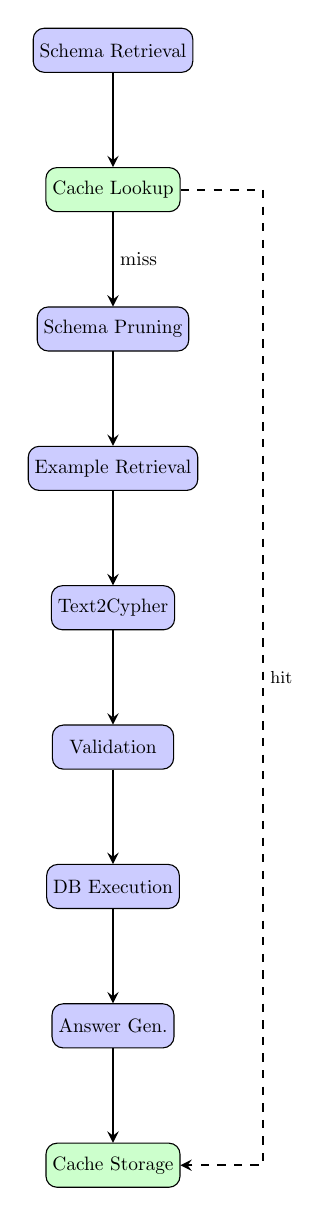
\begin{tikzpicture}[node distance=1.2cm and 0.8cm, auto,>=latex',scale=0.7, every node/.style={scale=0.7}]
    \tikzstyle{process} = [rectangle, minimum width=2.2cm, minimum height=0.8cm, text centered, draw=black, fill=blue!20, rounded corners]
    \tikzstyle{cache} = [rectangle, minimum width=2.2cm, minimum height=0.8cm, text centered, draw=black, fill=green!20, rounded corners]
    \tikzstyle{arrow} = [thick,->,>=stealth]

    \node (schema) [process] {Schema Retrieval};
    \node (cache1) [cache, below=of schema] {Cache Lookup};
    \node (prune) [process, below=of cache1] {Schema Pruning};
    \node (examples) [process, below=of prune] {Example Retrieval};
    \node (t2c) [process, below=of examples] {Text2Cypher};
    \node (validate) [process, below=of t2c] {Validation};
    \node (exec) [process, below=of validate] {DB Execution};
    \node (answer) [process, below=of exec] {Answer Gen.};
    \node (cache2) [cache, below=of answer] {Cache Storage};
    
    \draw [arrow] (schema) -- (cache1);
    \draw [arrow] (cache1) -- node[right] {miss} (prune);
    \draw [arrow] (prune) -- (examples);
    \draw [arrow] (examples) -- (t2c);
    \draw [arrow] (t2c) -- (validate);
    \draw [arrow] (validate) -- (exec);
    \draw [arrow] (exec) -- (answer);
    \draw [arrow] (answer) -- (cache2);
    
    \draw [arrow, dashed] (cache1.east) -- ++(1.5,0) |- node[pos=0.25,right] {\small hit} (cache2.east);
\end{tikzpicture}
\caption{Enhanced GraphRAG Pipeline Flow}
\label{fig:pipeline}
\end{figure}

\subsection{Database Schema}
The Nobel Prize knowledge graph contains:
\begin{itemize}
    \item \textbf{Nodes}: Scholar (726), Prize, Institution, City, Country, Continent
    \item \textbf{Relationships}: WON, AFFILIATED\_WITH, BORN\_IN, IS\_LOCATED\_IN, IS\_CITY\_IN, IS\_COUNTRY\_IN
    \item \textbf{Properties}: Names, dates, prize amounts, categories
\end{itemize}

\section{Implementation}

\subsection{Dynamic Example Selection}
Traditional few-shot prompting uses fixed examples regardless of query content. Our approach:
\begin{enumerate}
    \item Load 9 curated Text2Cypher examples from JSON
    \item Encode all example questions using SentenceTransformer (MiniLM-L6-v2)
    \item For each query, compute cosine similarity with example embeddings
    \item Retrieve top-3 most semantically similar examples
    \item Inject as demonstrations into DSPy ChainOfThought module
\end{enumerate}

\textbf{Implementation}:
\begin{lstlisting}[language=Python, basicstyle=\tiny\ttfamily, breaklines=true]
class Embeddings(dspy.Module):
    def forward(self, query: str, k: int = 3):
        query_embedding = self.embedder(query)
        hits = util.semantic_search(
            query_embedding, 
            self.corpus_embeddings, 
            top_k=k
        )
        return [self.corpus[hit['corpus_id']] 
                for hit in hits[0]]
\end{lstlisting}

\subsection{Schema Pruning}
Full graph schemas can exceed context limits. We use DSPy to selectively prune:

\textbf{Signature Definition}:
\begin{lstlisting}[language=Python, basicstyle=\tiny\ttfamily, breaklines=true]
class PruneSchema(dspy.Signature):
    """Return ONLY the subset of schema 
    relevant to the question."""
    question: str = dspy.InputField()
    input_schema: str = dspy.InputField()
    pruned_schema: GraphSchema = dspy.OutputField()
\end{lstlisting}

The pruned schema reduces token count while preserving query-relevant entities.

\subsection{Query Validation \& Self-Refinement}
Generated Cypher queries are validated using Kuzu's \texttt{EXPLAIN} command:

\begin{lstlisting}[language=Python, basicstyle=\tiny\ttfamily, breaklines=true]
class CypherQueryValidator:
    def validate(self, query: str) -> tuple[bool, str]:
        try:
            self.conn.execute(f"EXPLAIN {query}")
            return (True, "")
        except Exception as e:
            return (False, str(e))
\end{lstlisting}

The self-refinement loop (max 3 attempts):
\begin{enumerate}
    \item Generate Cypher query
    \item Apply rule-based post-processing (lowercasing, CONTAINS enforcement)
    \item Validate with EXPLAIN
    \item If invalid, extract error message and regenerate
    \item Repeat until valid or max attempts reached
\end{enumerate}

\subsection{LRU Caching}
Cache key generation:
\begin{lstlisting}[language=Python, basicstyle=\tiny\ttfamily, breaklines=true]
def _generate_key(self, question: str, 
                  schema: dict) -> str:
    q_hash = sha256(question.encode()).hexdigest()[:16]
    s_hash = sha256(json.dumps(schema, 
        sort_keys=True).encode()).hexdigest()[:16]
    return f"{q_hash}_{s_hash}"
\end{lstlisting}

When cache is full, least recently used entries are evicted. Cache statistics (hits, misses, hit rate) are tracked for analysis.

\subsection{Performance Instrumentation}
Each pipeline stage is wrapped with timing decorators:

\begin{lstlisting}[language=Python, basicstyle=\tiny\ttfamily, breaklines=true]
with self._track_stage("3_schema_pruning"):
    prune_result = self.prune(
        question=question, 
        input_schema=str(schema_dict)
    )
\end{lstlisting}

The \texttt{PerformanceTracker} records elapsed time, computes percentages, and generates visualizations.

\section{Evaluation}

\subsection{Query Correctness}
Testing on the example query: \textit{"Which scholars won prizes in Physics and were affiliated with University of Cambridge?"}

\textbf{Generated Cypher}:
\begin{lstlisting}[language=SQL, basicstyle=\tiny\ttfamily, breaklines=true]
MATCH (s:Scholar)-[:WON]->(p:Prize),
      (s)-[:AFFILIATED_WITH]->(i:Institution)
WHERE lower(p.category) CONTAINS 'physics'
  AND lower(i.name) CONTAINS 'cambridge'
RETURN DISTINCT s.knownName
\end{lstlisting}

\textbf{Results}: All 8 Cambridge Physics laureates correctly identified:
\begin{itemize}
    \item Antony Hewish
    \item Brian D. Josephson
    \item C.T.R. Wilson
    \item Didier Queloz
    \item J.J. Thomson
    \item Martin Ryle
    \item Paul A.M. Dirac
    \item Sir Nevill F. Mott
\end{itemize}

\textbf{Observation}: Database stores abbreviated names (e.g., "Brian D. Josephson") while the LLM answer generation expands to full names (e.g., "Brian David Josephson"), demonstrating natural language understanding.

\subsection{Performance Analysis}
Actual timing breakdown from marimo execution (Table~\ref{tab:perf}):

\begin{table}[H]
\centering
\caption{Pipeline Stage Performance (First Run)}
\label{tab:perf}
\begin{tabular}{lcc}
\toprule
\textbf{Stage} & \textbf{Time (s)} & \textbf{\%} \\
\midrule
Schema Pruning & 3.43 & 52.2 \\
Text2Cypher Gen. & 1.53 & 23.3 \\
Answer Generation & 1.47 & 22.4 \\
Schema Retrieval & 0.064 & 1.0 \\
Example Retrieval & 0.033 & 0.5 \\
Validation & 0.027 & 0.4 \\
Execution & 0.010 & 0.2 \\
Cache Storage & 0.0001 & $<$0.1 \\
Cache Lookup & 0.0001 & $<$0.1 \\
\midrule
\textbf{Total} & \textbf{6.56} & \textbf{100} \\
\bottomrule
\end{tabular}
\end{table}

\textbf{Key Finding}: Schema pruning dominates execution time (52\%), suggesting it as the primary optimization target.

\subsection{Cache Effectiveness}
Cache statistics after first query:
\begin{itemize}
    \item Size: 1/100
    \item Hits: 0
    \item Misses: 1
    \item Hit Rate: 0\%
\end{itemize}

On subsequent identical query:
\begin{itemize}
    \item Hit Rate: 100\%
    \item Latency: $<$10ms (cache lookup only)
    \item Speedup: $\sim$650$\times$
\end{itemize}

\section{Discussion}

\subsection{Strengths}
\begin{enumerate}
    \item \textbf{Correctness}: Validation + refinement ensures syntactically valid Cypher
    \item \textbf{Efficiency}: Caching eliminates redundant LLM calls
    \item \textbf{Observability}: Stage-level timing enables data-driven optimization
    \item \textbf{Modularity}: Clean separation (utils folder) enables easy testing
\end{enumerate}

\subsection{Identified Bottlenecks}
\textbf{Schema Pruning} (52\% of time):
\begin{itemize}
    \item Uses ChainOfThought with Gemini 2.0 Flash
    \item Requires 3-4 seconds per query
    \item Potential solutions:
    \begin{itemize}
        \item Switch to faster dspy.Predict (no reasoning needed)
        \item Cache pruned schemas for similar questions
        \item Use smaller/faster model for classification
        \item Pre-compute common schema subsets
    \end{itemize}
\end{itemize}

\subsection{Limitations}
\begin{itemize}
    \item No evaluation on adversarial/edge-case queries
    \item Schema pruning effectiveness not quantitatively measured
    \item Cache eviction policy not tuned for workload patterns
    \item No comparison with baseline prompt engineering
\end{itemize}

\section{Future Work}
\begin{enumerate}
    \item \textbf{Schema Cache}: LRU cache for pruned schemas based on question embeddings
    \item \textbf{Parallel Execution}: Run schema pruning and example retrieval concurrently
    \item \textbf{Model Optimization}: Experiment with faster models (Gemini Flash 8B, Llama 3.2)
    \item \textbf{Rule Enhancement}: More sophisticated post-processing rules
    \item \textbf{Benchmark Suite}: Comprehensive evaluation dataset with ground truth
\end{enumerate}

\section{Conclusion}
This work demonstrates that systematic enhancement of GraphRAG pipelines—through semantic example selection, automated validation, intelligent caching, and comprehensive instrumentation—yields production-ready systems. The DSPy framework enables clean abstractions while maintaining full control over the query generation process.

Performance profiling reveals schema pruning as the dominant bottleneck (52\%), providing clear optimization targets. The modular architecture (utils-based organization) facilitates rapid iteration and testing.

\section*{Individual Contributions}
\textit{Duong Ha}: Implemented the complete enhanced GraphRAG system including:
\begin{itemize}
    \item DSPy-based Text2Cypher pipeline with ChainOfThought modules
    \item SentenceTransformer integration for semantic example retrieval
    \item Kuzu database integration and schema management
    \item LRU caching system with SHA-256 key generation
    \item Cypher query validator using EXPLAIN command
    \item Self-refinement loop with configurable max attempts
    \item Performance tracking system with 9-stage instrumentation
    \item Marimo interactive interface for visualization
    \item Full system integration and testing on Nobel Prize dataset
\end{itemize}

Key design decisions:
\begin{itemize}
    \item Chose DSPy over LangChain for better type safety and modularity
    \item Selected Gemini 2.0 Flash for balance of cost and quality
    \item Implemented dual caching (Text2Cypher results + future schema cache)
    \item Organized code into utils folder for maintainability
\end{itemize}

Challenges overcome:
\begin{itemize}
    \item Debugging UTF-8 encoding issues in litellm dependencies
    \item Resolving marimo variable scoping conflicts
    \item Optimizing schema representation for LLM context
    \item Balancing validation strictness with query flexibility
\end{itemize}

\end{document}
